\cotefile{79}
\scanpage{283}

\[
\begin{aligned}
(s,t)\in A_0&\Longleftrightarrow(s,\lambda t)\in A_\lambda\\
\mathrm{Et}_{A_0}(t)&=\mathrm{Et}_{A_\lambda}(\lambda t)
\end{aligned}
\]

\figure{\begin{tikzpicture}[x=.88cm,y=.78cm]
\draw (0,0)--(1,0) (1.6,0)--(3.15,0);
\draw (2.5,1.9) .. controls (3.65,.8) and (3.45,-1.35) .. (2.43,-2.0);
\draw[->] (2.85,1.10)..controls (3.44,0) and (3.2,-1.53)..(2.43,-2.0);
\draw (3.53,.13)--(6.69,1.95) (3.68,-.49)..controls (4.59,-1.10) and (5.81,-1.80)..(6.69,-1.93);
\draw (7.42,2.56)..controls (5.82,1.63) and (5.55,-2.04)..(7.83,-2.62);
\draw[->] (6.14,.15)..controls (6.19,1.11) and (6.43,1.65)..(6.70,1.94);
\draw (6.22,.05)--(8.18,0);
\foreach \x/\y in {0/0,2.5/1.9,2.43/-2,3.15/0,3.44/.14,6.22/.05,6.69/1.95,6.69/-1.93,8.18/0}{\fill (\x,\y) circle (1.15pt);}
\node[below right] at (-.1,0) {$\sigma t$}; \node at (1.35,0) {$s$};
\node[above] at (2.60,1.92) {$t'$}; \node[below right] at (2.40,-1.9) {$t''$};
\node at (3.49,-.05) {$t$}; \node[left] at (6.22,.05) {$\lambda t$};
\node[above left] at (6.78,2.02) {$t'$}; \node[below left] at (6.81,-1.89) {$t''$};
\node[right] at (8.18,0) {$\underset{\substack{\shortparallel\\s'}}{\lambda^{-1}s}$};
\draw[->] (4.00,3.10)--node[above] {$\lambda$} node[below] {$u_\lambda$} (5.04,3.10);
\draw[<-] (3.84,-2.54)--node[above] {$\lambda^{-1}$} node[below] {$u_{\lambda^{-1}}$} (5.07,-2.54);
\draw[->] (9.12,-.02)--(11.16,-.02); \draw[->] (10.10,-.18)..controls (10.25,.06) and (10.23,.30)..(10.15,.49);
\node at (.25,1.56) {$\checkmark$};
\end{tikzpicture}}

\[t'=\lambda t\dotplus\unsure{\nu|v}\ \big/\ t''=\lambda t-\nu\]

% margin note written sideways
\margin{$R_0\subset S\times S^*$}

\[\sigma(\lambda t)=\lambda\sigma(t)\quad\text{lié à }t\]

\figure{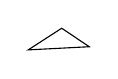
\begin{tikzpicture}[scale=.5]\draw (0,0)--(.85,.55)--(1.55,.08)--cycle;\end{tikzpicture}}

\[(s,t)\in A_0\Longleftrightarrow(s,\lambda t)\in A_\lambda\]

\[
\begin{aligned}
&\forall a,\ \unsure{\exists!|\exists}f\ \text{triangle, tel que}\quad a\in f\\
&\deleted{N/6}\ \operatorname{card} A=N/2\\
&\operatorname{card} F=(N/2)!
\end{aligned}
\]

$(a,f)$ en nb $\nu\,(N/2)$

donc il y a $\nu(N/2)/3$ faces

Si $\nu=1$, ça fait $N/6$ faces

\uline{le stabilisateur d'une face serait d'ordre $6$}

\figure{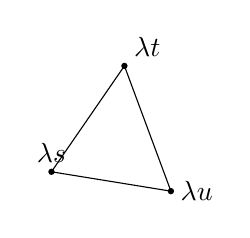
\begin{tikzpicture}[scale=.82]
\draw (0,0)--(1.13,1.64)--(1.85,-.30)--cycle;
\foreach \x/\y in {0/0,1.13/1.64,1.85/-.30}{\fill (\x,\y) circle (1.4pt);}
\node[above] at (0,0) {$\lambda s$};\node[above right] at (1.13,1.64) {$\lambda t$};
\node[right] at (1.85,-.30) {$\lambda u$};
\end{tikzpicture}}

\[\boxed{\lambda t\underset{\substack{s'\\\shortparallel\\\lambda^{-1}s}}{\overset{\cdot}{\pm}}\nu\ \text{est incident à }t}\]

\[
\begin{aligned}
\lambda(t\underset{s}{\dotplus}\zeta)\pm\nu&\ \text{est incident : }t+\zeta\\
\lambda t\underset{s'}{\dotplus}\underbrace{\lambda^2\zeta\pm\nu}&\ \rule{2cm}{.3pt}\ t+\zeta\\
\zeta'&=\lambda^2\zeta\pm\nu\\
\zeta&=\lambda^{-2}\zeta'\pm\lambda^{-2}\cdot\nu
\end{aligned}
\]

\[\lambda^{-2}\nu=\nu^{-1}\]

% margin note written sideways
\margin{\unsure{irréelle|ivréelle} \deleted{dans} au beau milieu de ce délire mathématico-philoso}

% archive sheet number: 282
